\documentclass[xcolor={table}]{beamer}
\mode<presentation>{
  \usetheme{Boadilla}
  \usefonttheme[onlylarge]{structurebold}
  \usefonttheme[stillsansseriflarge]{serif}
  \setbeamerfont*{frametitle}{size=\normalsize,series=\bfseries}
  % \setbeamertemplate{navigation symbols}{}
  \setbeamercovered{transparent}
}
\usepackage[english]{babel}
\usepackage[latin1]{inputenc}
\usepackage{times}
\usepackage[T1]{fontenc}
\usepackage{amsmath}
\usepackage{amssymb}
\usepackage{esint}
\usepackage{hyperref}
\usepackage{tikz}
\usepackage{xkeyval}
\usepackage{xargs}
\usepackage{verbatim}
\usepackage{listings}
\usepackage{multimedia}
\newcommand\hmmax{0}
\newcommand\bmmax{0}
\usepackage{bm}
\usepackage{siunitx}
\usepackage{xcolor,pifont}
\usepackage{upgreek}

\usetikzlibrary{
  arrows,
  calc,
  decorations.pathmorphing,
  decorations.pathreplacing,
  decorations.markings,
  fadings,
  positioning,
  shapes,
  arrows.meta
}
\usepgfmodule{oo}

\pgfdeclareradialshading{glow2}{\pgfpoint{0cm}{0cm}}{
  color(0mm)=(white);
  color(2mm)=(white);
  color(8mm)=(black);
  color(10mm)=(black)
}
\pgfdeclareradialshading{glow}{\pgfpoint{0cm}{0cm}}{
  color(0mm)=(white);
  color(5mm)=(white);
  color(9mm)=(black);
  color(10mm)=(black)
}

\begin{tikzfadingfrompicture}[name=glow fading]
  \shade [shading=glow] (0,0) circle (1);
\end{tikzfadingfrompicture}

\begin{tikzfadingfrompicture}[name=glow2 fading]
  \shade [shading=glow2] (0,0) circle (1);
\end{tikzfadingfrompicture}

\mode<handout>{
  \usepackage{pgfpages}
  \pgfpagesuselayout{4 on 1}[a4paper,landscape,border shrink=5mm]
  \setbeamercolor{background canvas}{bg=black!10}
}

\newcommand\pgfmathsinandcos[3]{%
  \pgfmathsetmacro#1{sin(#3)}%
  \pgfmathsetmacro#2{cos(#3)}%
}
\newcommand\LongitudePlane[3][current plane]{%
  \pgfmathsinandcos\sinEl\cosEl{#2} % elevation
  \pgfmathsinandcos\sint\cost{#3} % azimuth
  \tikzset{#1/.estyle={cm={\cost,\sint*\sinEl,0,\cosEl,(0,0)}}}
}
\newcommand\LatitudePlane[3][current plane]{%
  \pgfmathsinandcos\sinEl\cosEl{#2} % elevation
  \pgfmathsinandcos\sint\cost{#3} % latitude
  \pgfmathsetmacro\yshift{\cosEl*\sint}
  \tikzset{#1/.estyle={cm={\cost,0,0,\cost*\sinEl,(0,\yshift)}}} %
}
\newcommand\DrawLongitudeCircle[2][1]{
  \LongitudePlane{\angEl}{#2}
  \tikzset{current plane/.prefix style={scale=#1}}
  % angle of "visibility"
  \pgfmathsetmacro\angVis{atan(sin(#2)*cos(\angEl)/sin(\angEl))} %
  \draw[current plane] (\angVis:1) arc (\angVis:\angVis+180:1);
  \draw[current plane,dashed] (\angVis-180:1) arc (\angVis-180:\angVis:1);
}
\newcommand\DrawLatitudeCircleArrow[2][1]{
  \LatitudePlane{\angEl}{#2}
  \tikzset{current plane/.prefix style={scale=#1}}
  \pgfmathsetmacro\sinVis{sin(#2)/cos(#2)*sin(\angEl)/cos(\angEl)}
  % angle of "visibility"
  \pgfmathsetmacro\angVis{asin(min(1,max(\sinVis,-1)))}
  \draw[current plane,decoration={markings, mark=at position 0.6 with {\arrow{<}}},postaction={decorate},line width=.6mm] (\angVis:1) arc (\angVis:-\angVis-180:1);
  \draw[current plane,dashed,line width=.6mm] (180-\angVis:1) arc (180-\angVis:\angVis:1);
}
\newcommand\DrawLatitudeCircle[2][1]{
  \LatitudePlane{\angEl}{#2}
  \tikzset{current plane/.prefix style={scale=#1}}
  \pgfmathsetmacro\sinVis{sin(#2)/cos(#2)*sin(\angEl)/cos(\angEl)}
  % angle of "visibility"
  \pgfmathsetmacro\angVis{asin(min(1,max(\sinVis,-1)))}
  \draw[current plane] (\angVis:1) arc (\angVis:-\angVis-180:1);
  \draw[current plane,dashed] (180-\angVis:1) arc (180-\angVis:\angVis:1);
}
\newcommand\coil[1]{
  {\rh * cos(\t * pi r)}, {\apart * (2 * #1 + \t) + \rv * sin(\t * pi r)}
}
\makeatletter
\define@key{DrawFromCenter}{style}[{->}]{
  \tikzset{DrawFromCenterPlane/.style={#1}}
}
\define@key{DrawFromCenter}{r}[1]{
  \def\@R{#1}
}
\define@key{DrawFromCenter}{center}[(0, 0)]{
  \def\@Center{#1}
}
\define@key{DrawFromCenter}{theta}[0]{
  \def\@Theta{#1}
}
\define@key{DrawFromCenter}{phi}[0]{
  \def\@Phi{#1}
}
\presetkeys{DrawFromCenter}{style, r, center, theta, phi}{}
\newcommand*\DrawFromCenter[1][]{
  \setkeys{DrawFromCenter}{#1}{
    \pgfmathsinandcos\sint\cost{\@Theta}
    \pgfmathsinandcos\sinp\cosp{\@Phi}
    \pgfmathsinandcos\sinA\cosA{\angEl}
    \pgfmathsetmacro\DX{\@R*\cost*\cosp}
    \pgfmathsetmacro\DY{\@R*(\cost*\sinp*\sinA+\sint*\cosA)}
    \draw[DrawFromCenterPlane] \@Center -- ++(\DX, \DY);
  }
}
\newcommand*\DrawFromCenterText[2][]{
  \setkeys{DrawFromCenter}{#1}{
    \pgfmathsinandcos\sint\cost{\@Theta}
    \pgfmathsinandcos\sinp\cosp{\@Phi}
    \pgfmathsinandcos\sinA\cosA{\angEl}
    \pgfmathsetmacro\DX{\@R*\cost*\cosp}
    \pgfmathsetmacro\DY{\@R*(\cost*\sinp*\sinA+\sint*\cosA)}
    \draw[DrawFromCenterPlane] \@Center -- ++(\DX, \DY) node {#2};
  }
}
\makeatother

% not mandatory, but I though it was better to set it blank
\setbeamertemplate{headline}{}
\def\beamer@entrycode{\vspace{-\headheight}}

\tikzstyle{snakearrow} = [decorate, decoration={pre length=0.2cm,
  post length=0.2cm, snake, amplitude=.4mm,
  segment length=2mm},thick, ->]

%% document-wide tikz options and styles

\tikzset{%
  % >=latex, % option for nice arrows
  inner sep=0pt,%
  outer sep=2pt,%
  mark coordinate/.style={inner sep=0pt,outer sep=0pt,minimum size=3pt,
    fill=black,circle}%
}
\tikzset{
  % Define standard arrow tip
  >=stealth',
  % Define style for boxes
  punkt/.style={
    rectangle,
    rounded corners,
    draw=black, very thick,
    text width=8em,
    minimum height=2.5em,
    text centered},
}

\tikzset{onslide/.code args={<#1>#2}{%
    \only<#1>{\pgfkeysalso{#2}}
    % \pgfkeysalso doesn't change the path
  }}
\tikzset{alt/.code args={<#1>#2#3}{%
    \alt<#1>{\pgfkeysalso{#2}}{\pgfkeysalso{#3}}
    % \pgfkeysalso doesn't change the path
  }}
\tikzset{temporal/.code args={<#1>#2#3#4}{%
    \temporal<#1>{\pgfkeysalso{#2}}{\pgfkeysalso{#3}}{\pgfkeysalso{#4}}
    % \pgfkeysalso doesn't change the path
  }}

\makeatletter
\newbox\@backgroundblock
\newenvironment{backgroundblock}[2]{%
  \global\setbox\@backgroundblock=\vbox\bgroup%
  \unvbox\@backgroundblock%
  \vbox to0pt\bgroup\vskip#2\hbox to0pt\bgroup\hskip#1\relax%
}{\egroup\egroup\egroup}
\addtobeamertemplate{background}{\box\@backgroundblock}{}
\makeatother

\newcommand{\ud}{\mathrm{d}}
\newcommand{\ue}{\mathrm{e}}
\newcommand{\ui}{\mathrm{i}}
\newcommand{\Na}{\mathrm{Na}}
\newcommand{\Cs}{\mathrm{Cs}}
\newcommand{\abs}[1]{{\left|{#1}\right|}}
\newcommand{\paren}[1]{{\left({#1}\right)}}

% \def\timeleft{15:00->14:55}

\title{Demonstration of the trapped-ion quantum CCD computer architecture}
\date{May 5, 2021}
\author{Yichao Yu}
\institute{Ni Group}

\ifpdf
% Ensure reproducible output
\pdfinfoomitdate=1
\pdfsuppressptexinfo=-1
\pdftrailerid{}
\hypersetup{
  pdfcreator={},
  pdfproducer={}
}
\fi

\begin{document}

\begin{frame}{}
  \titlepage
\end{frame}

% * QCCD
% * Requirement
% % * Use movement for scalability
% % * Dual species
% % * Formally ...
% * Device: (requirement 1)
% % * a 1-D tube with electrodes along the axial
% % * Beam parallel to device surface
% % * Single zone addressing
% * Transport (requirement 2)
% % * DC electrodes
% % * 1-D: require swapping (local 2-D)
% % * Cooling after transport
% * Cooling (requirement 4)
% * Phase tracking (requirement 3)
% % * Stable qubit and stable drive
% * Parallelized operation (requirement 5)
% % * Holistic benchmarks
% * QV Test

\begin{frame}{}
  \begin{center}
    \begin{columns}
      \column{9cm}
      \begin{itemize}
      \item QCCD
      \item Requirements
      \item Solutions and benchmarks
      \end{itemize}
    \end{columns}
  \end{center}
\end{frame}

\begin{frame}{QCCD}
  \begin{center}
    \begin{columns}
      \column{8cm}
      \begin{center}
        Quantum Charge Coupled Device:\\\vspace{0.5cm}
        \uncover<2->{i.e. moving charges around}
      \end{center}
    \end{columns}
  \end{center}
\end{frame}

\begin{frame}{Scalable quantum computing platform}
  \begin{center}
    \begin{tikzpicture}
      \node[draw,red,rounded corners=.2cm,inner sep=0.12cm,align=center] (L1) at (-4, 2)
      {Control of\\multiple qubits};
      \node[draw,green!50!black,rounded corners=.2cm,inner sep=0.12cm,align=center]
      (L2) at (-4, 0) {Multi-qubits gates};
      \node[draw,blue,rounded corners=.2cm,inner sep=0.12cm,align=center] (L3) at (-4, -2)
      {High fidelity\\operations};

      \visible<2->{
        \node[draw,red,rounded corners=.2cm,inner sep=0.12cm,align=center] (R1) at (4, 3)
        {Trapping\\multiple ions};
        \draw[red,->,>=stealth,line width=1] (L1) -- (R1);
      }

      \visible<3->{
        \node[draw,green!50!black,rounded corners=.2cm,inner sep=0.12cm,align=center]
        (R2) at (4, 1.5) {Ion transport};
        \draw[green!50!black,->,>=stealth,line width=1] (L2) -- (R2);
      }

      \visible<4->{
        \node[draw,alt=<4>{green!50!black}{green!50!blue},rounded corners=.2cm,
        inner sep=0.12cm,align=center] (R3) at (4, 0) {Cooling};
        \draw[green!50!black,->,>=stealth,line width=1] (L2) -- (R3);
        \draw[green!50!black,->,>=stealth,line width=1] (R2) -- (R3);
      }

      \visible<5->{
        \draw[blue,->,>=stealth,line width=1] (L3) -- (R3);
      }

      \visible<6->{
        \node[draw,blue,rounded corners=.2cm,inner sep=0.12cm,align=center] (R4) at (4, -1.5)
        {Phase tracking};
        \draw[blue,->,>=stealth,line width=1] (L3) -- (R4);
      }

      \visible<7->{
        \node[draw,green!50!blue,rounded corners=.2cm,inner sep=0.12cm,align=center]
        (R5) at (4, -3) {Parallel\\operation};
        \draw[green!50!black,->,dashed,>=stealth,line width=1] (L2) -- (R5);
        \draw[blue,->,dashed,>=stealth,line width=1] (L3) -- (R5);
      }
    \end{tikzpicture}
  \end{center}
\end{frame}

\begin{frame}{Device}
  \begin{center}
    \begin{tikzpicture}
      \node at (0, 0) {
\includegraphics[width=8cm]{setup}};
    \end{tikzpicture}
  \end{center}
\end{frame}

\begin{frame}{Gate operation and transport}
  \begin{center}
    \begin{tikzpicture}
      \node at (0, 0) {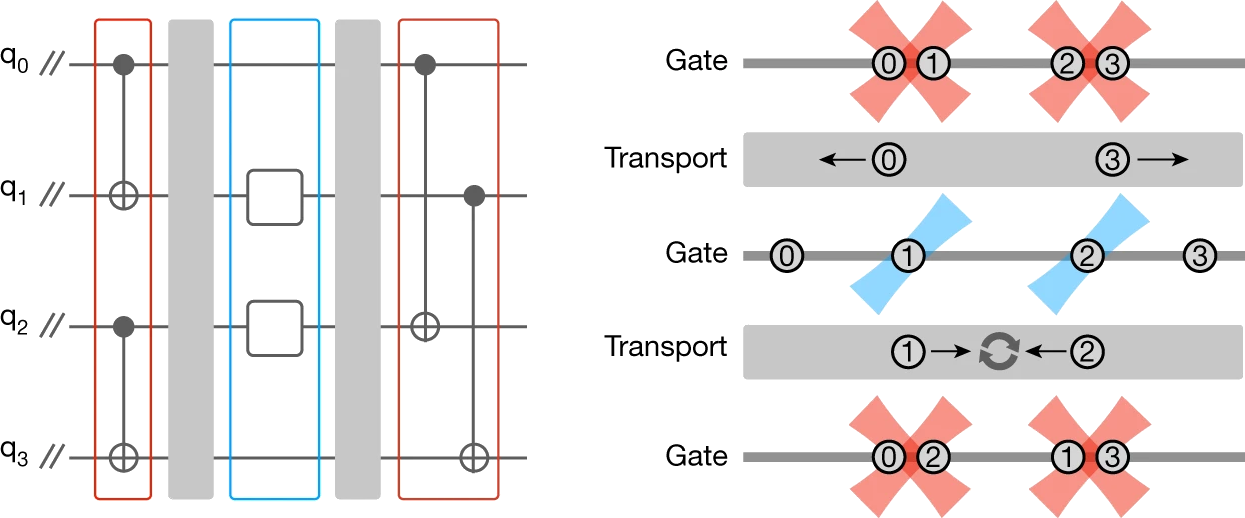
\includegraphics[width=7cm]{sequence}};
      \visible<2->{
        \node[text width=6cm] at (0, -3) {
          \begin{itemize}
          \item Swapping
          \item<3-> Cooling with $^{138}\mathrm{Ba}^+$
          \item<4-> Low crosstalk
          \end{itemize}
        };
      }
    \end{tikzpicture}
  \end{center}
\end{frame}

\begin{frame}{Quantum Volume}
  \begin{center}
    \begin{tikzpicture}
      \node at (0, 0) {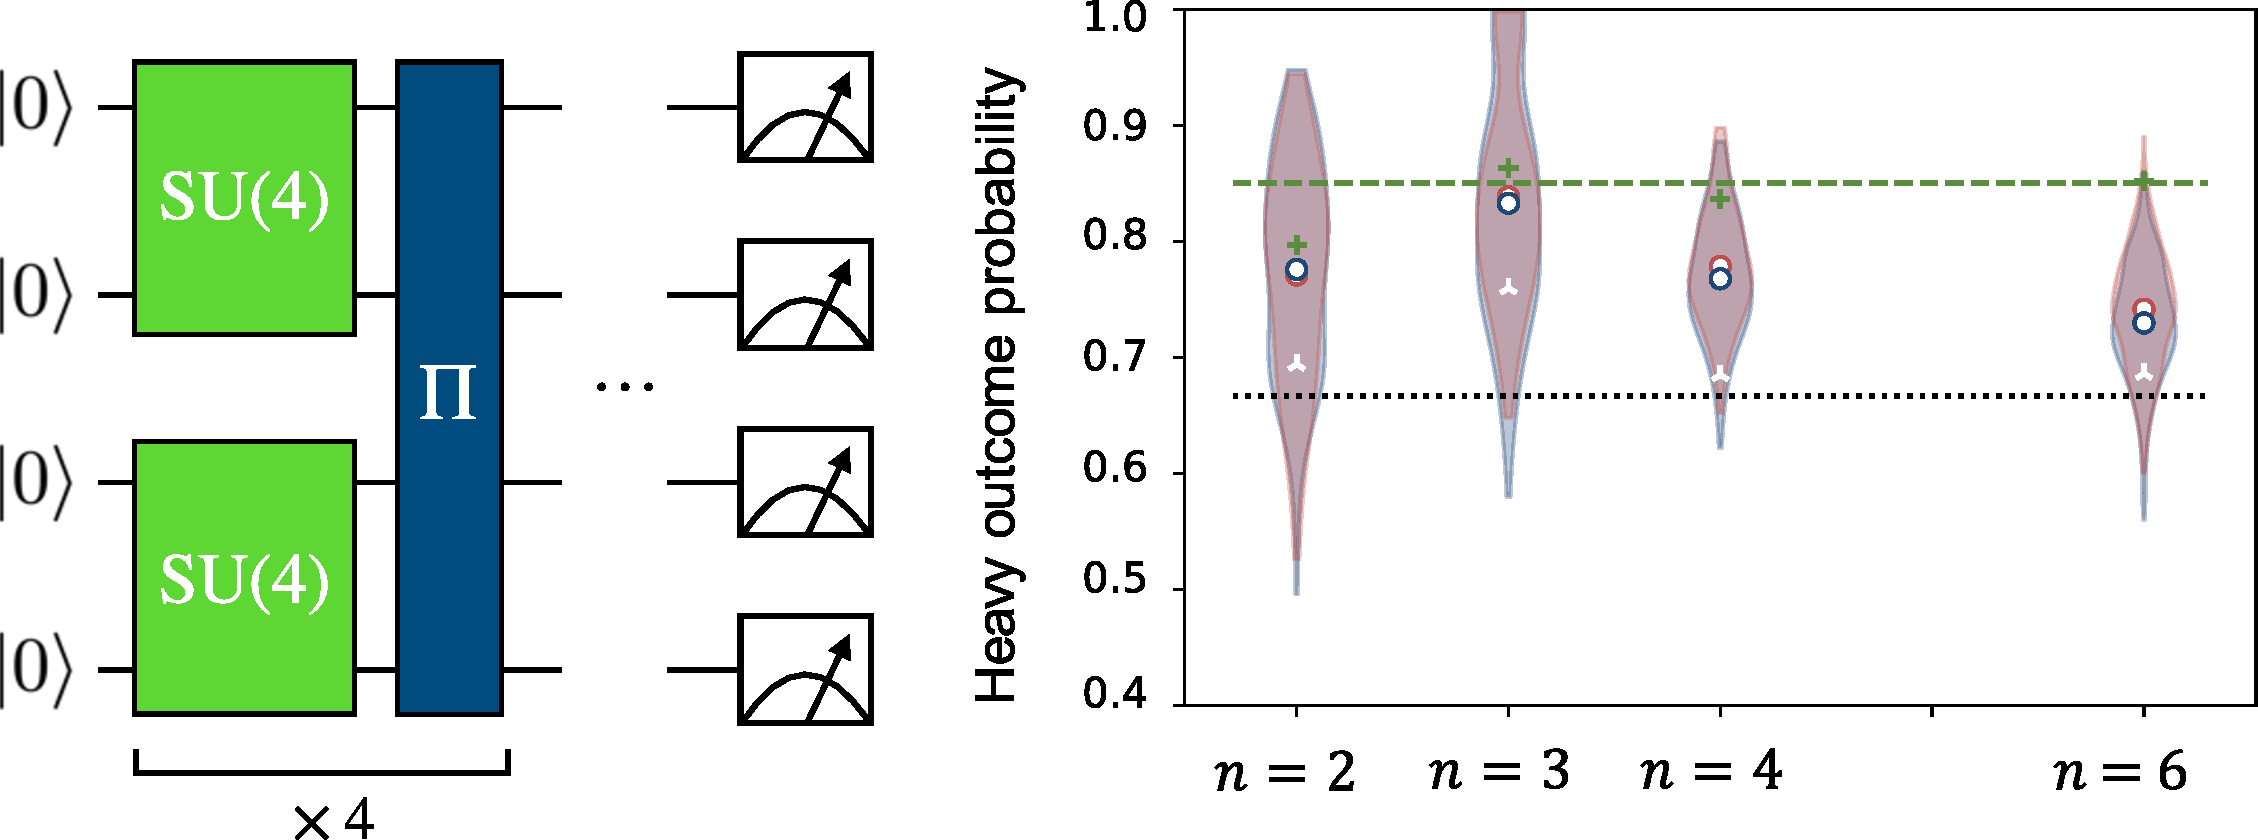
\includegraphics[width=7cm]{QV}};
    \end{tikzpicture}
  \end{center}
\end{frame}

\end{document}
